\chapter{Measured improvements}
\label{sec:improvements}

After implementing the transformations, we measure the effectiveness of the new normalization strategy. We look at the results from the perspective of submission coverage and normalization effectiveness.

\section{Submission coverage}

Recall that Ask-Elle considers two programs to be semantically equivalent if their normal forms are syntactically similar. Additionally, a program is considered correct if it is equivalent to one of the model solutions.

While it is possible to have two model solutions that share the same normal form, this does not increase the amount of programs that are recognized. In such a case, removing one of the model solutions would have no impact.

If we only consider model solutions with different normal forms, we can associate each of them to a different cluster of programs. If the submissions to an exercise are grouped in 10 clusters, then having 10 model solutions (one per cluster) would recognize 100\% of programs.

With \emph{submission coverage}, we measure the percentage of programs that are recognized using 5 model solutions or less. Figures \ref{fig:improvements-coverage-1} through \ref{fig:improvements-coverage-8} show graphs for each exercise. The circle shows the percentage of solutions originally recognized by Ask-Elle and the cross shows the same measurement after our improvements. Notice how additional model solutions offers diminishing returns.

\begin{figure}
\centering
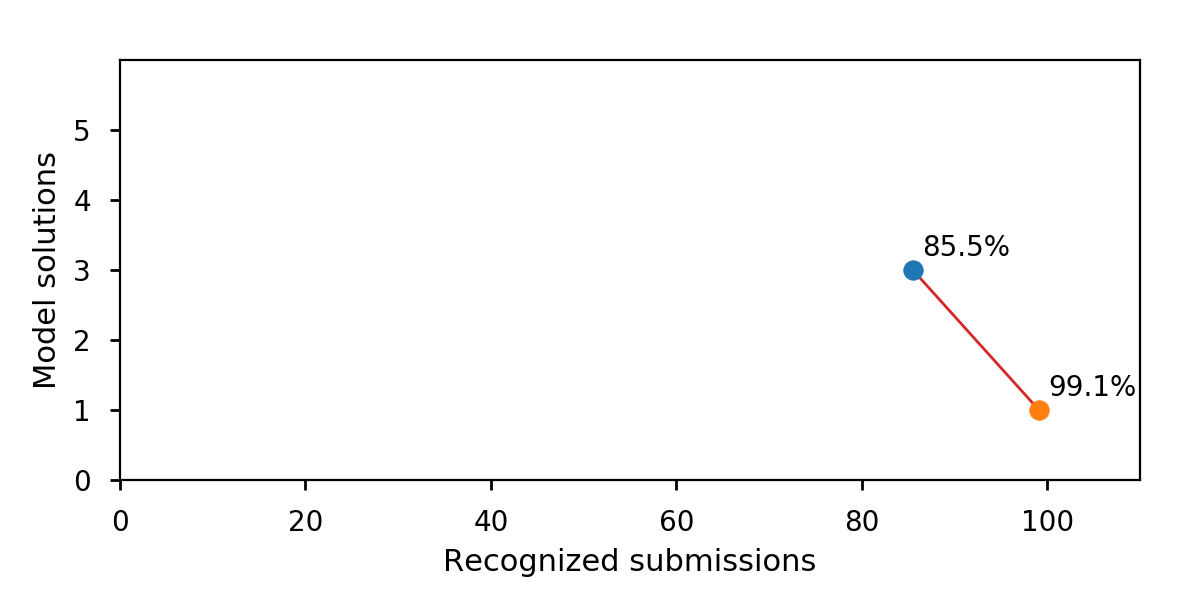
\includegraphics[height=10cm]{graphs/coverage-1.png}
\caption{Exercise 1 - Improvement in submission coverage}
\label{fig:improvements-coverage-1}
\end{figure}

\begin{figure}
\centering
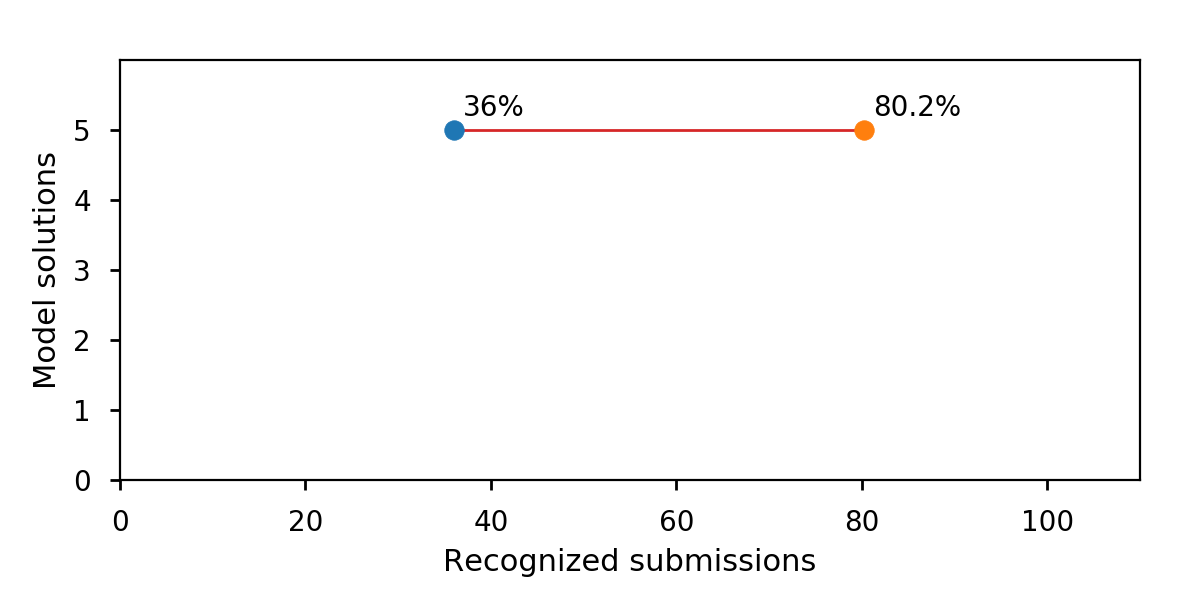
\includegraphics[height=10cm]{graphs/coverage-2.png}
\caption{Exercise 2 - Improvement in submission coverage}
\label{fig:improvements-coverage-2}
\end{figure}

\begin{figure}
\centering
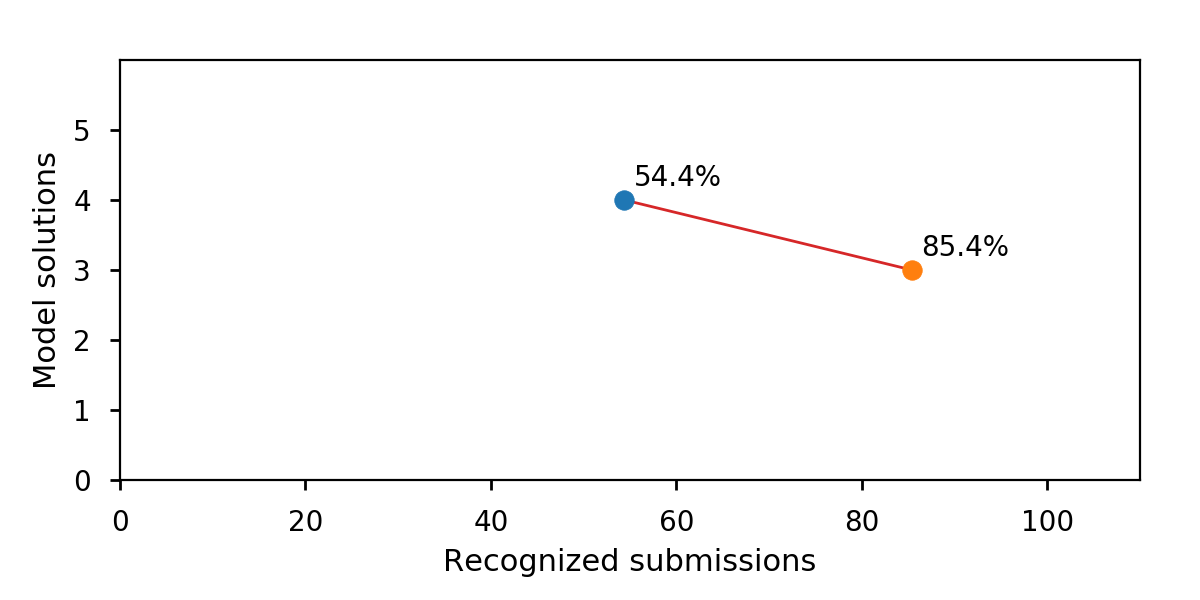
\includegraphics[height=10cm]{graphs/coverage-3.png}
\caption{Exercise 3 - Improvement in submission coverage}
\label{fig:improvements-coverage-3}
\end{figure}

\begin{figure}
\centering
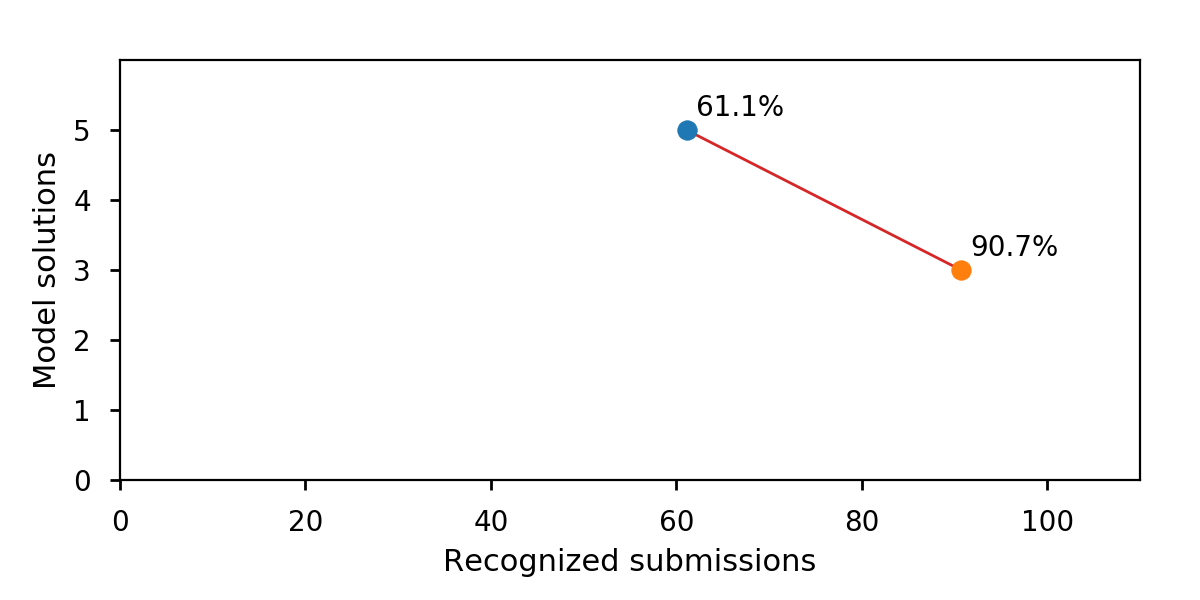
\includegraphics[height=10cm]{graphs/coverage-4.png}
\caption{Exercise 4 - Improvement in submission coverage}
\label{fig:improvements-coverage-4}
\end{figure}

\begin{figure}
\centering
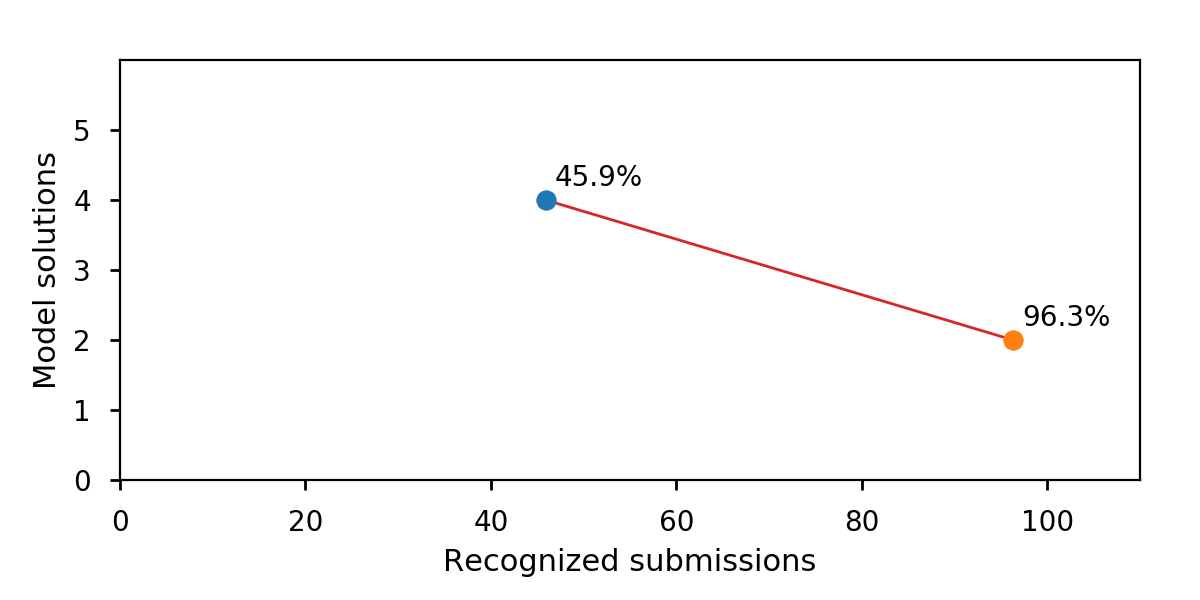
\includegraphics[height=10cm]{graphs/coverage-5.png}
\caption{Exercise 5 - Improvement in submission coverage}
\label{fig:improvements-coverage-5}
\end{figure}

\begin{figure}
\centering
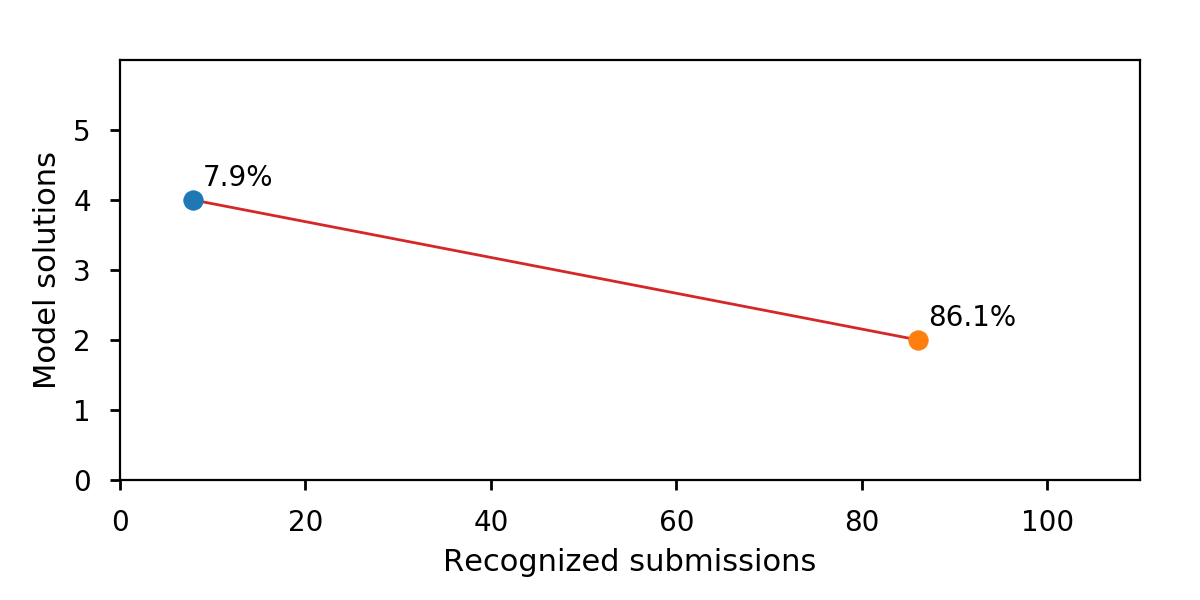
\includegraphics[height=10cm]{graphs/coverage-6.png}
\caption{Exercise 6 - Improvement in submission coverage}
\label{fig:improvements-coverage-6}
\end{figure}

\begin{figure}
\centering
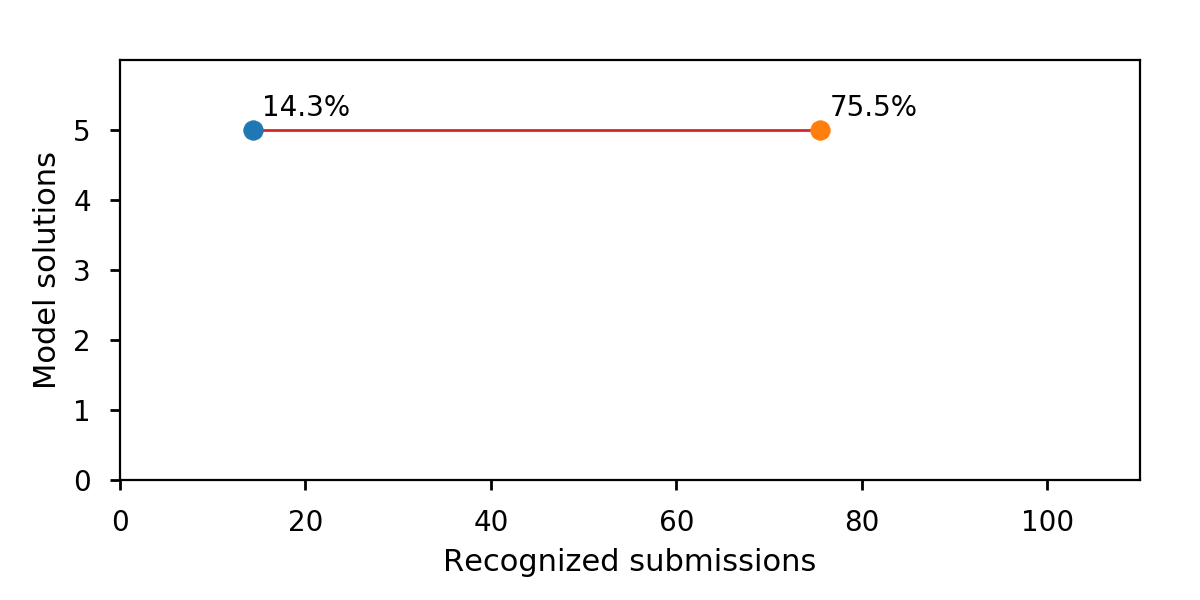
\includegraphics[height=10cm]{graphs/coverage-7.png}
\caption{Exercise 7 - Improvement in submission coverage}
\label{fig:improvements-coverage-7}
\end{figure}

\begin{figure}
\centering
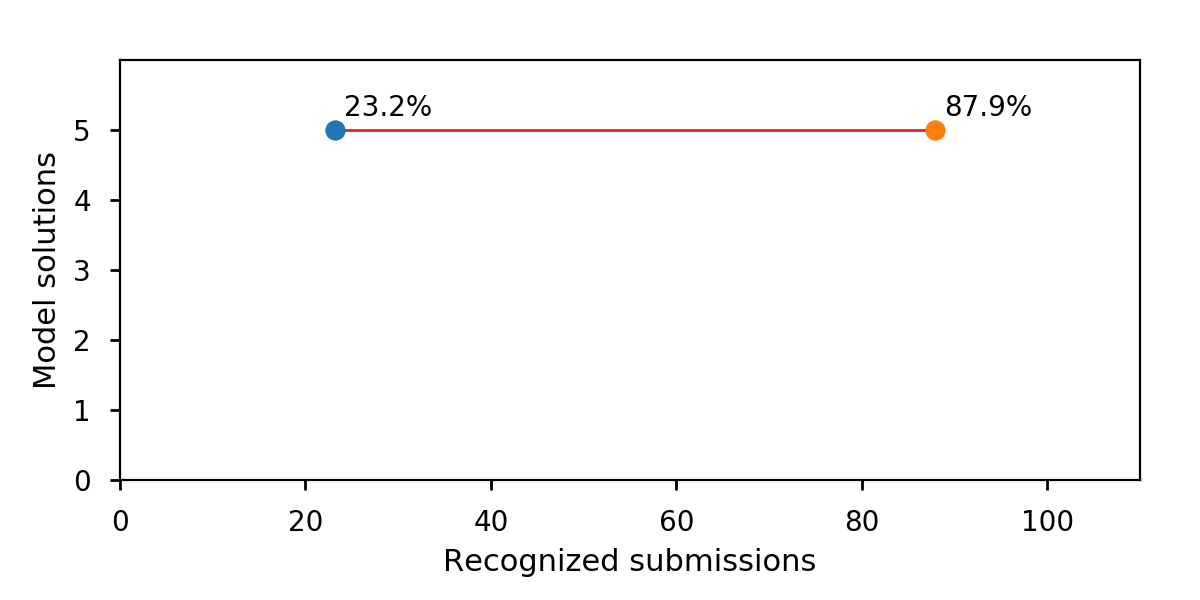
\includegraphics[height=10cm]{graphs/coverage-8.png}
\caption{Exercise 8 - Improvement in submission coverage}
\label{fig:improvements-coverage-8}
\end{figure}

\section{Normalization effectiveness}

As mentioned in \ref{sec:method-measurement-definitions}, we say that a given normalization procedure is more effective than a second one when it results in a lower amount of clusters for the same exercise. Our results show that, for all exercises, the new normalization is more effective than Ask-Elle's original one.

Table \ref{tb:improvements-clusters} shows the amount of clusters per exercise. We also provide figures \ref{fig:improvements-clusters-1} through \ref{fig:improvements-clusters-8} that present the numbers in a more graphical way. Additionally, the figures show the differences in size of each cluster. Notice how the amount of clusters diminishes, while the size of the clusters grows.

\begin{table}
\centering
\begin{tabular}{ m{6em} | m{6em} | m{6em} }
Exercise & Before & After \\
\hline
1 & 15 & 2 \\
\hline
2 & 64 & 19 \\
\hline
3 & 43 & 16 \\
\hline
4 & 38 & 12 \\
\hline
5 & 43 & 6 \\
\hline
6 & 97 & 16 \\
\hline
7 & 84 & 28 \\
\hline
8 & 76 & 18
\end{tabular}
\caption{Improvement in normalization effectiveness}
\label{tb:improvements-clusters}
\end{table}

\begin{figure}
\centering
\begin{tabular}{ >{\centering\arraybackslash}m{14em} >{\centering\arraybackslash}m{14em} }
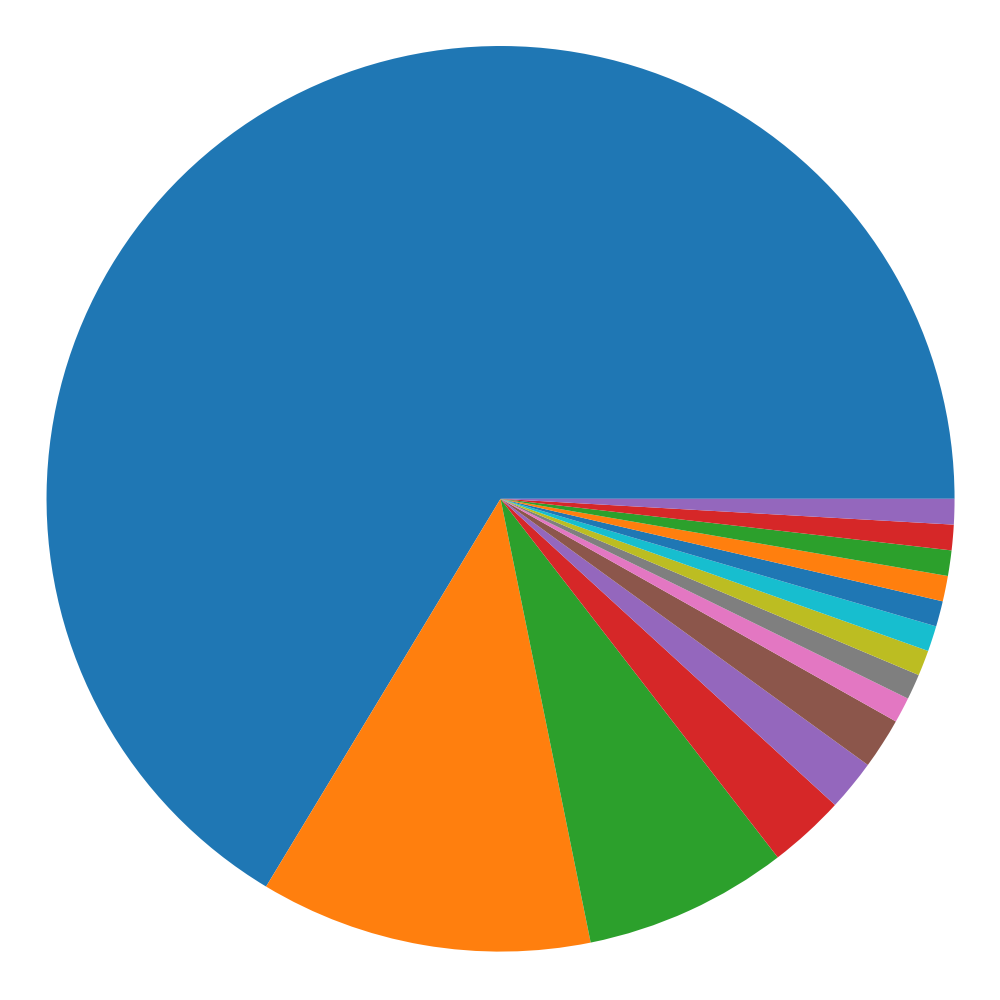
\includegraphics[height=5cm]{graphs/cluster-baseline-1.png}
&
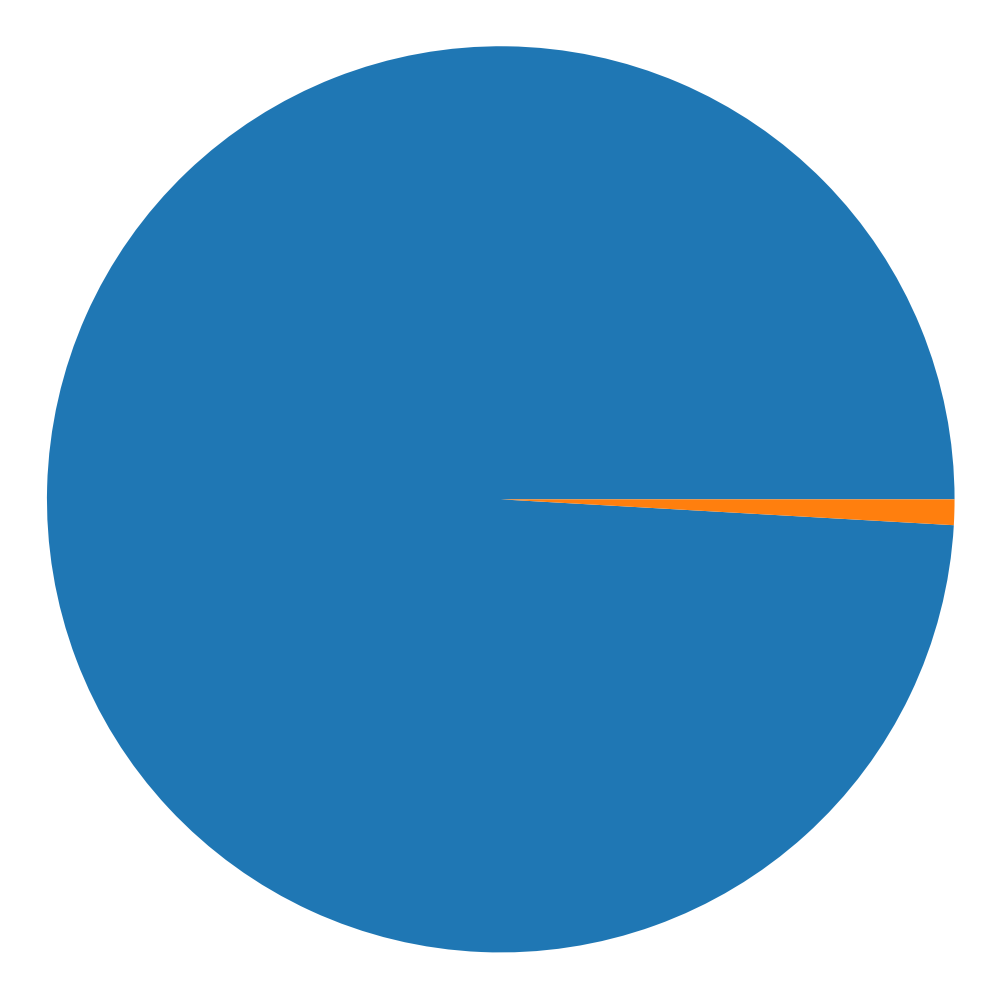
\includegraphics[height=5cm]{graphs/cluster-aggressive-1.png} \\
Before & After
\end{tabular}
\caption{Exercise 1 - Improvement in normalization effectiveness}
\label{fig:improvements-clusters-1}
\end{figure}

\begin{figure}
\centering
\begin{tabular}{ >{\centering\arraybackslash}m{14em} >{\centering\arraybackslash}m{14em} }
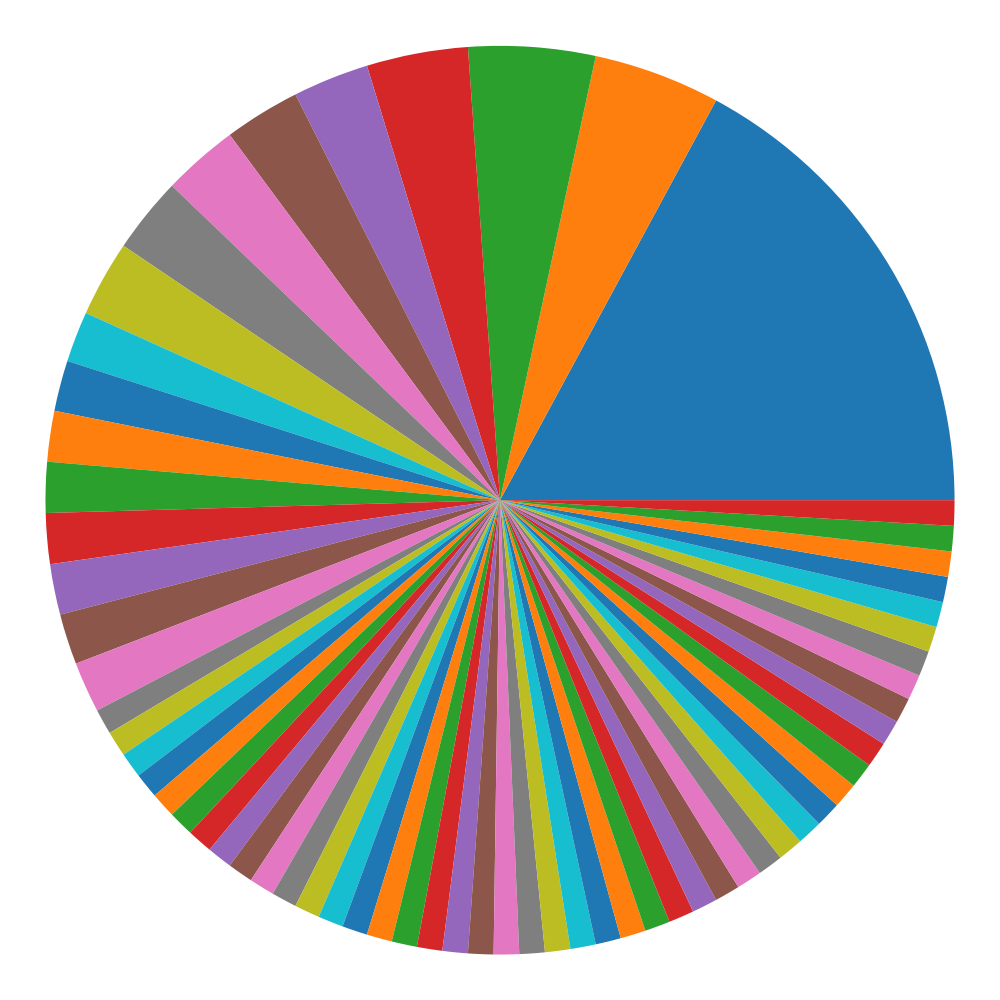
\includegraphics[height=5cm]{graphs/cluster-baseline-2.png}
&
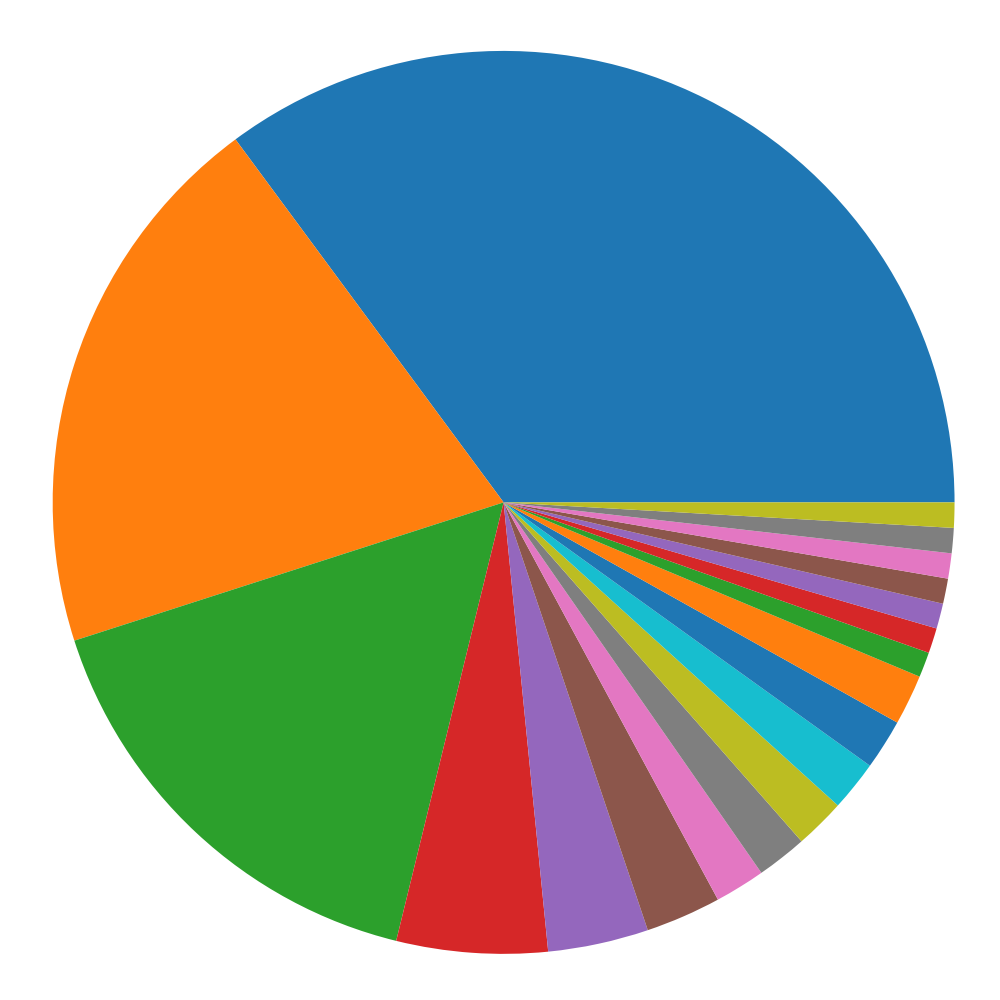
\includegraphics[height=5cm]{graphs/cluster-aggressive-2.png} \\
Before & After
\end{tabular}
\caption{Exercise 2 - Improvement in normalization effectiveness}
\label{fig:improvements-clusters-2}
\end{figure}

\begin{figure}
\centering
\begin{tabular}{ >{\centering\arraybackslash}m{14em} >{\centering\arraybackslash}m{14em} }
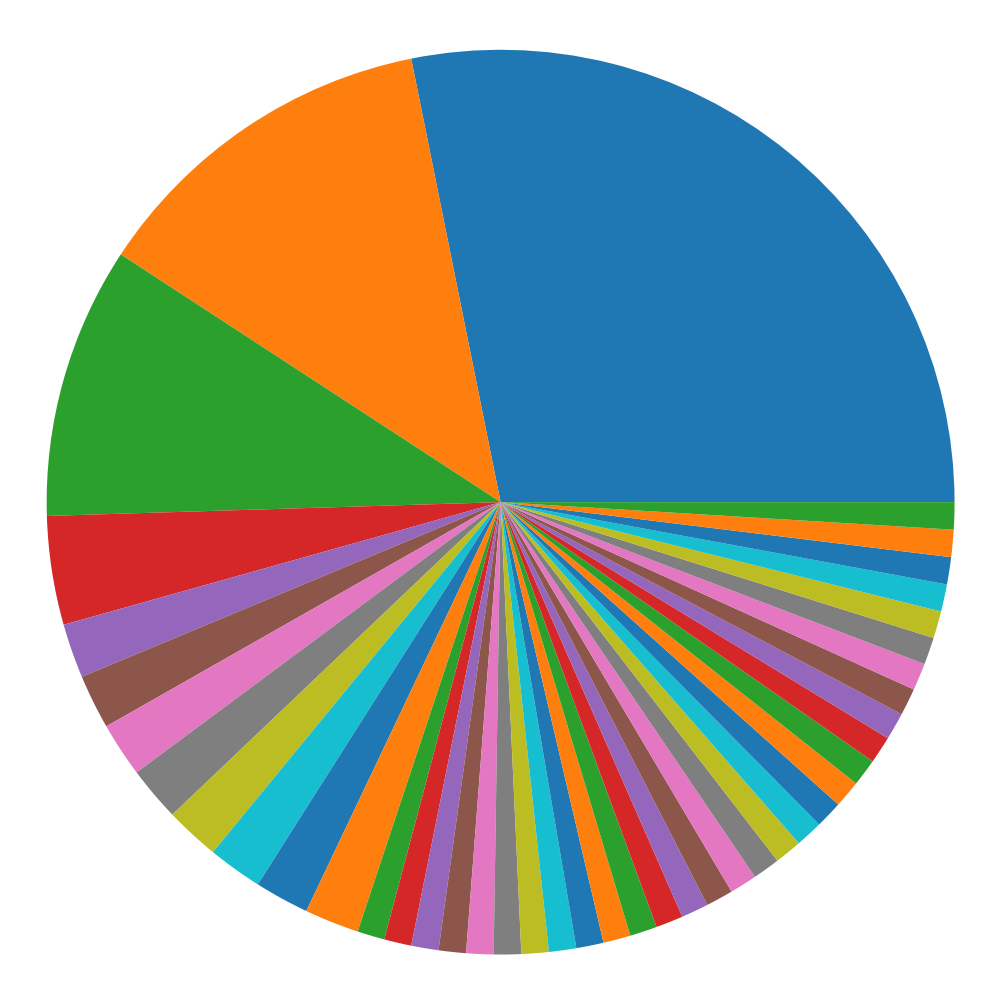
\includegraphics[height=5cm]{graphs/cluster-baseline-3.png}
&
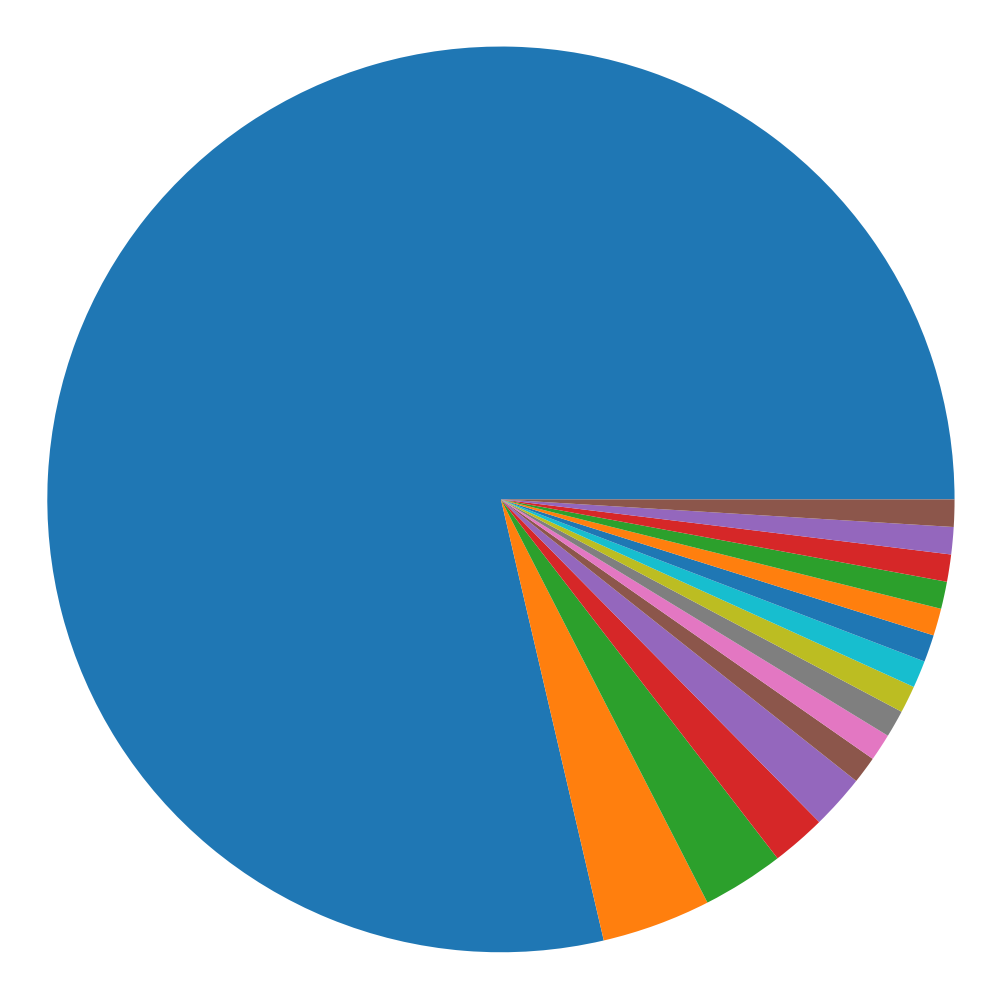
\includegraphics[height=5cm]{graphs/cluster-aggressive-3.png} \\
Before & After
\end{tabular}
\caption{Exercise 3 - Improvement in normalization effectiveness}
\label{fig:improvements-clusters-3}
\end{figure}

\begin{figure}
\centering
\begin{tabular}{ >{\centering\arraybackslash}m{14em} >{\centering\arraybackslash}m{14em} }
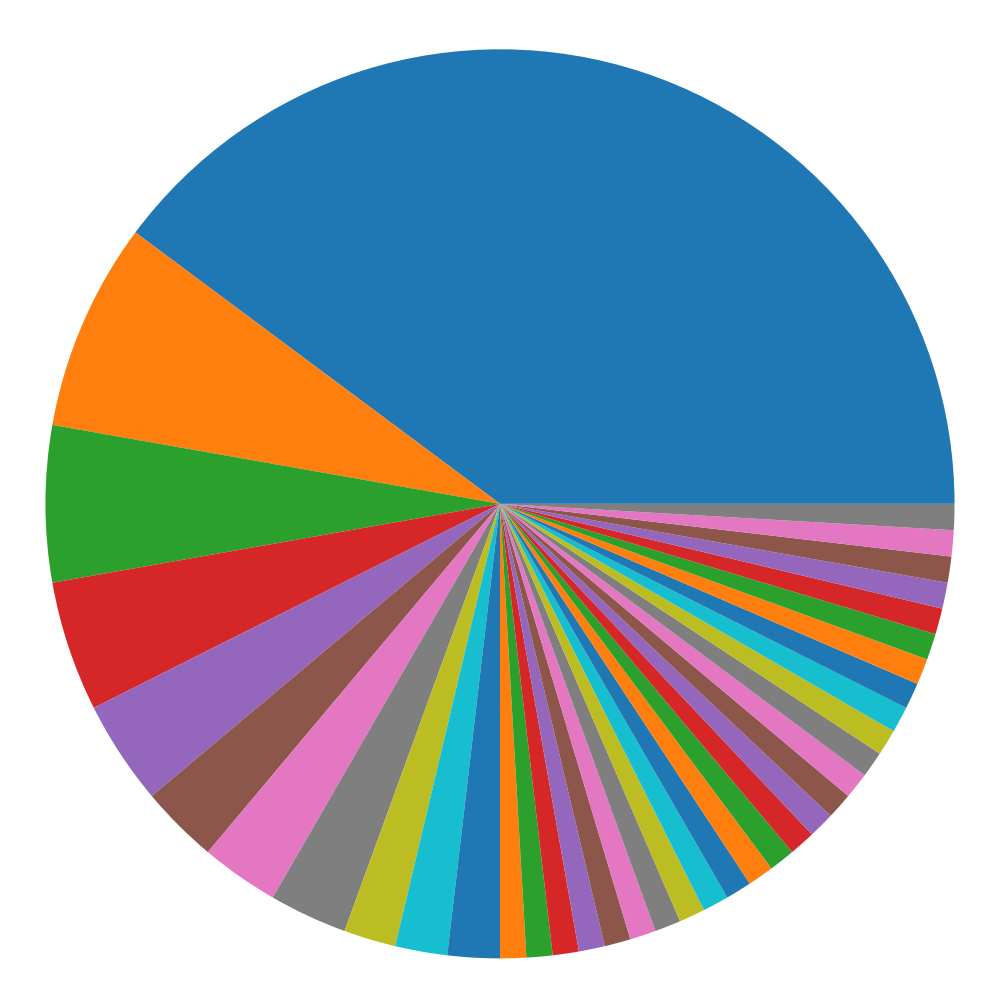
\includegraphics[height=5cm]{graphs/cluster-baseline-4.png}
&
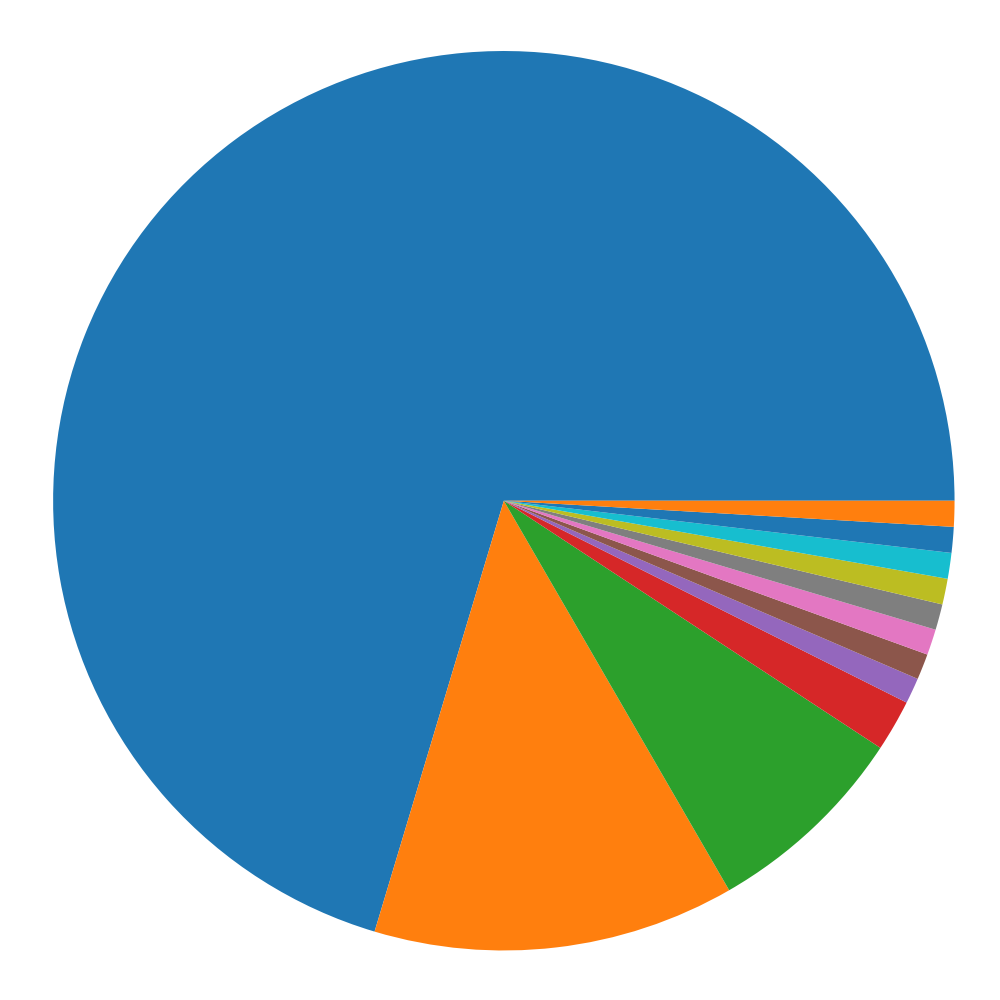
\includegraphics[height=5cm]{graphs/cluster-aggressive-4.png} \\
Before & After
\end{tabular}
\caption{Exercise 4 - Improvement in normalization effectiveness}
\label{fig:improvements-clusters-4}
\end{figure}

\begin{figure}
\centering
\begin{tabular}{ >{\centering\arraybackslash}m{14em} >{\centering\arraybackslash}m{14em} }
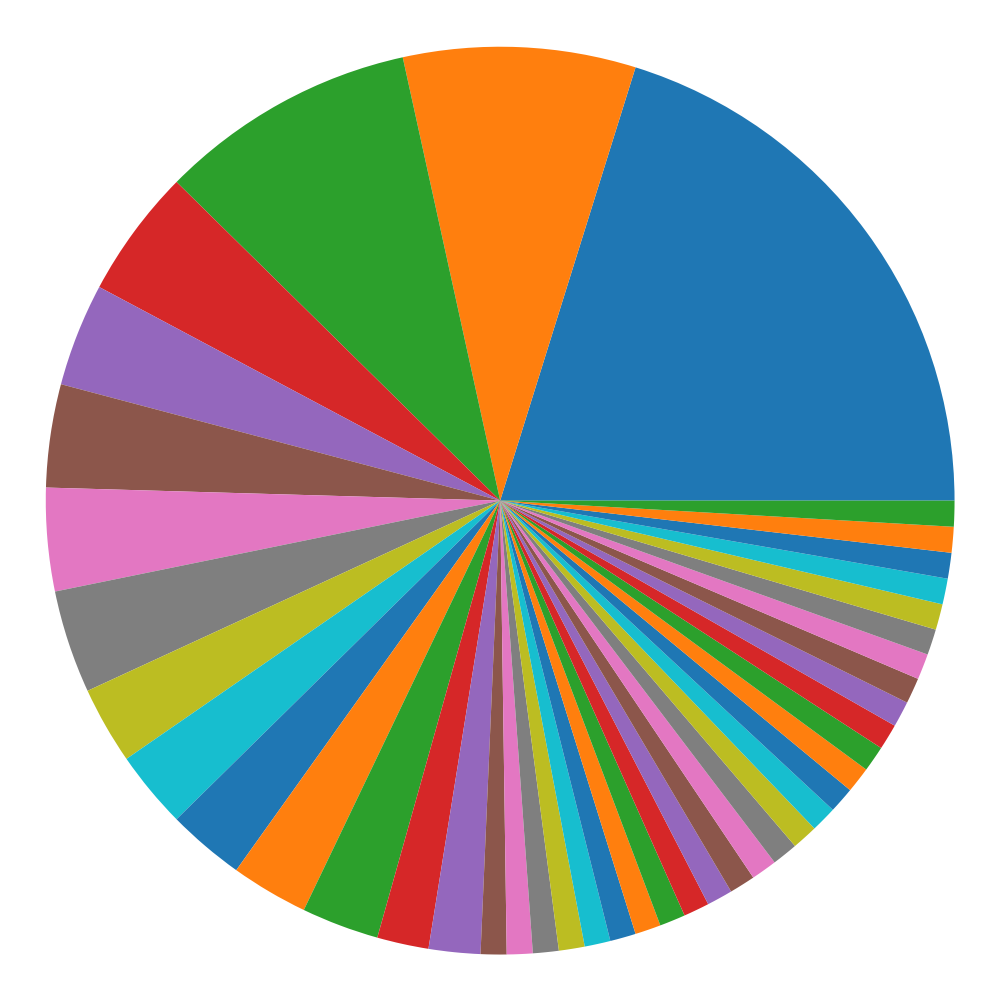
\includegraphics[height=5cm]{graphs/cluster-baseline-5.png}
&
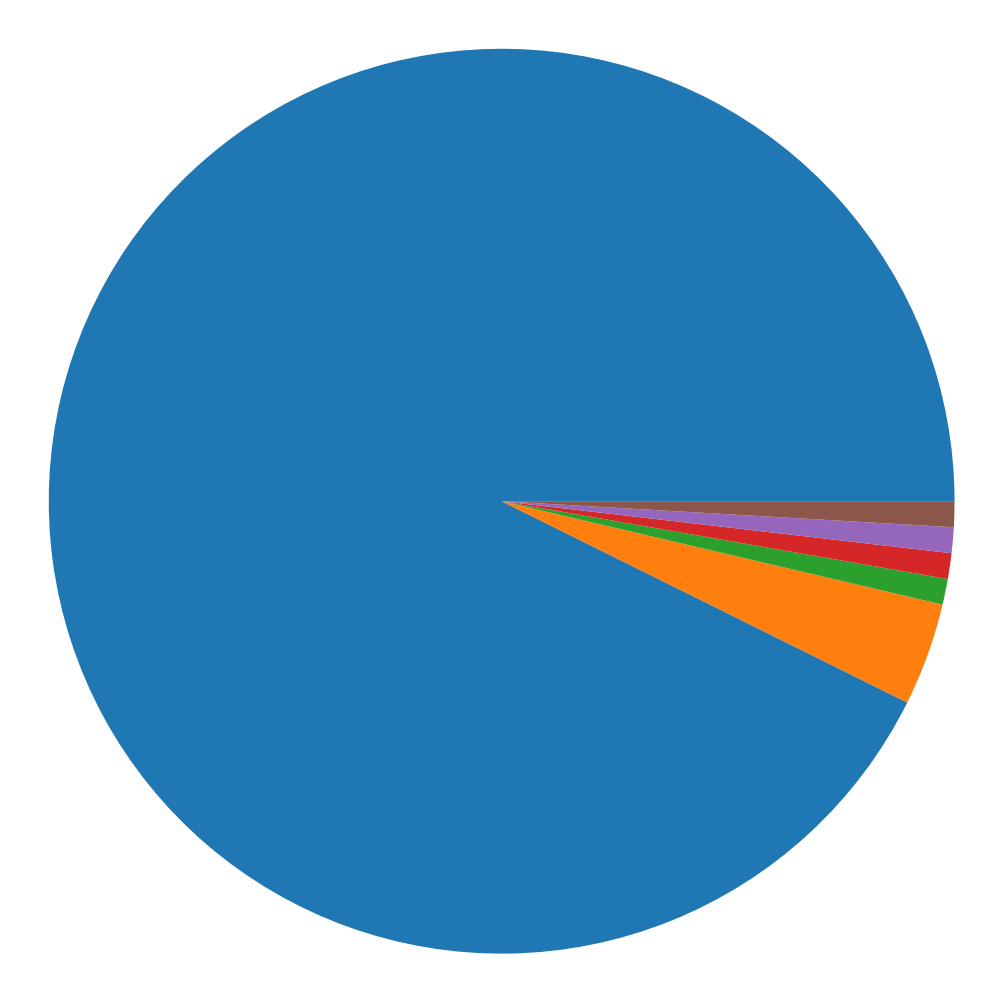
\includegraphics[height=5cm]{graphs/cluster-aggressive-5.png} \\
Before & After
\end{tabular}
\caption{Exercise 5 - Improvement in normalization effectiveness}
\label{fig:improvements-clusters-5}
\end{figure}

\begin{figure}
\centering
\begin{tabular}{ >{\centering\arraybackslash}m{14em} >{\centering\arraybackslash}m{14em} }
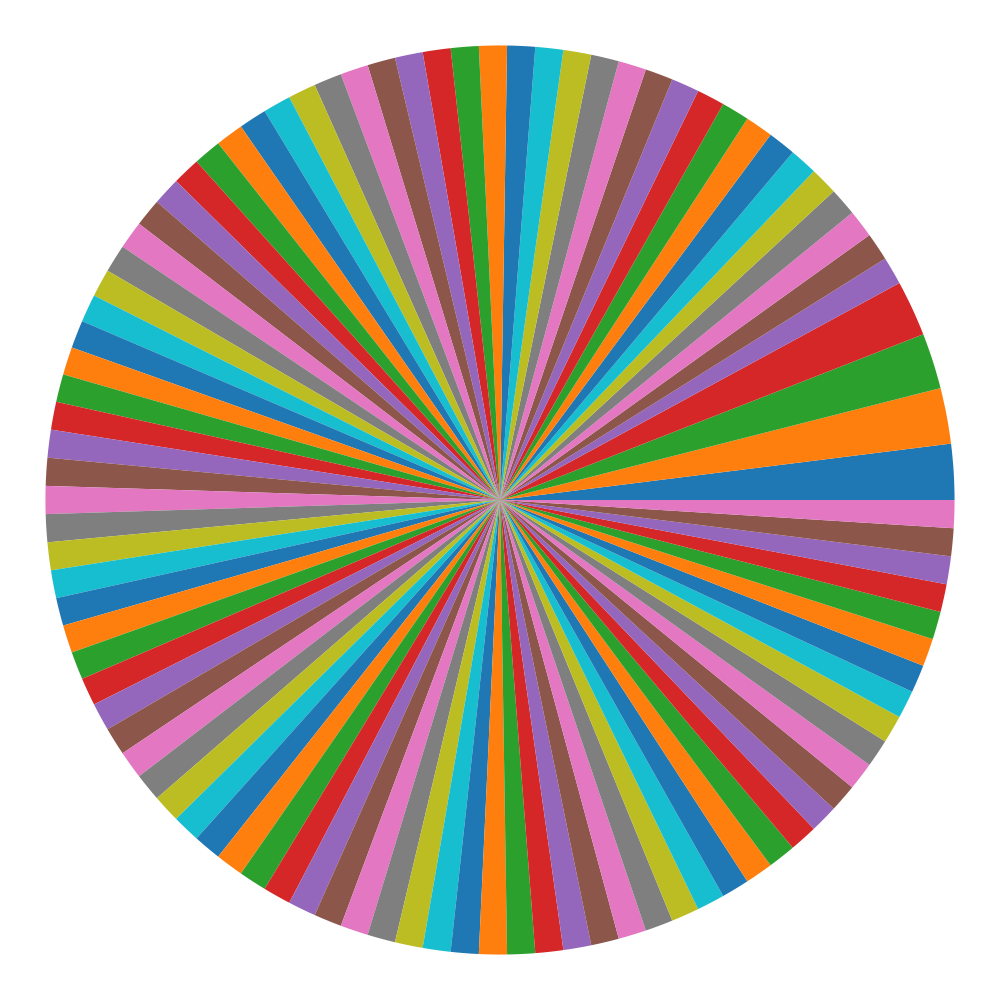
\includegraphics[height=5cm]{graphs/cluster-baseline-6.png}
&
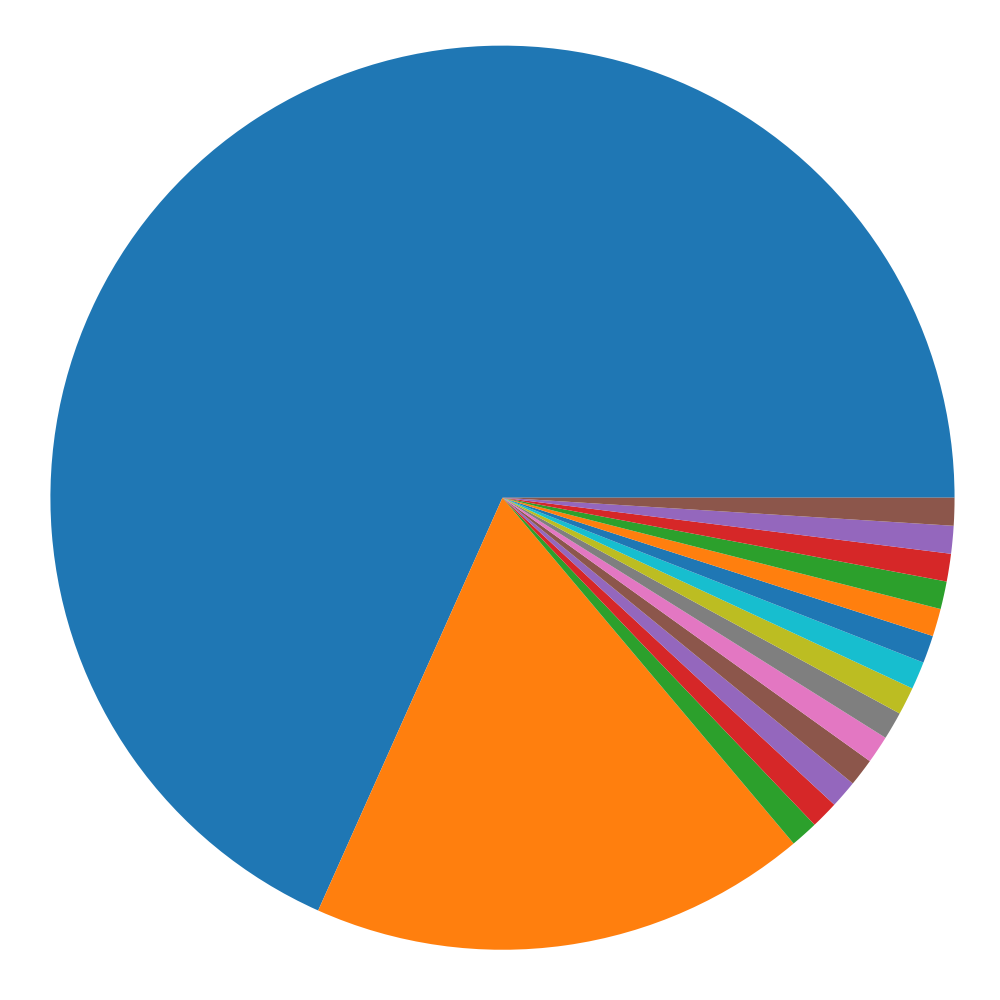
\includegraphics[height=5cm]{graphs/cluster-aggressive-6.png} \\
Before & After
\end{tabular}
\caption{Exercise 6 - Improvement in normalization effectiveness}
\label{fig:improvements-clusters-6}
\end{figure}

\begin{figure}
\centering
\begin{tabular}{ >{\centering\arraybackslash}m{14em} >{\centering\arraybackslash}m{14em} }
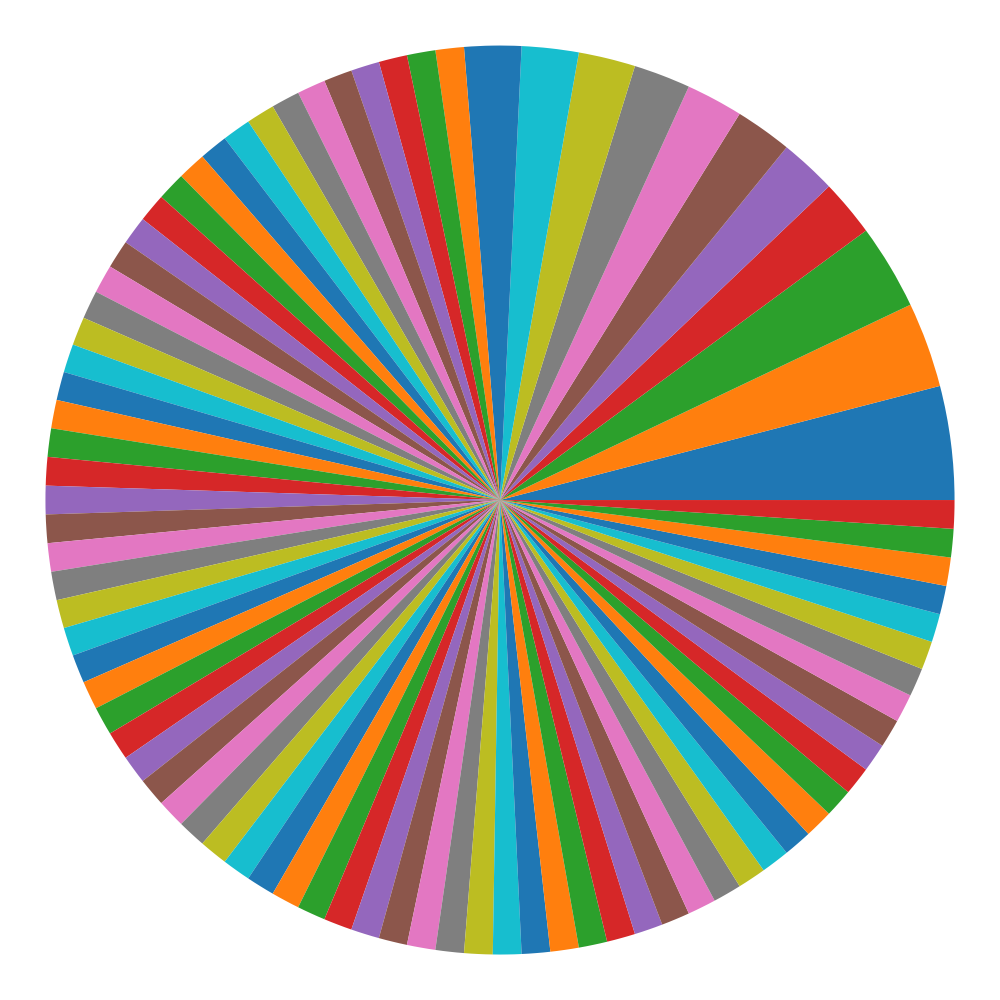
\includegraphics[height=5cm]{graphs/cluster-baseline-7.png}
&
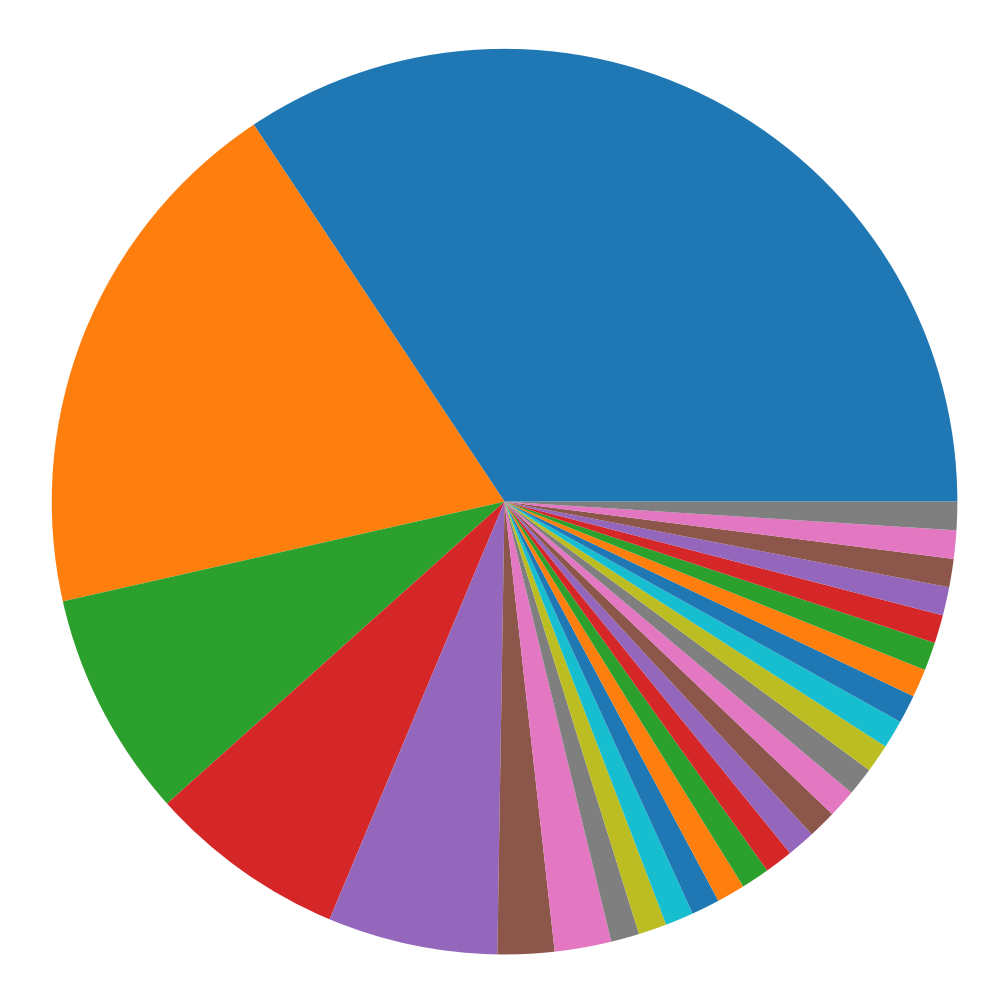
\includegraphics[height=5cm]{graphs/cluster-aggressive-7.png} \\
Before & After
\end{tabular}
\caption{Exercise 7 - Improvement in normalization effectiveness}
\label{fig:improvements-clusters-7}
\end{figure}

\begin{figure}
\centering
\begin{tabular}{ >{\centering\arraybackslash}m{14em} >{\centering\arraybackslash}m{14em} }
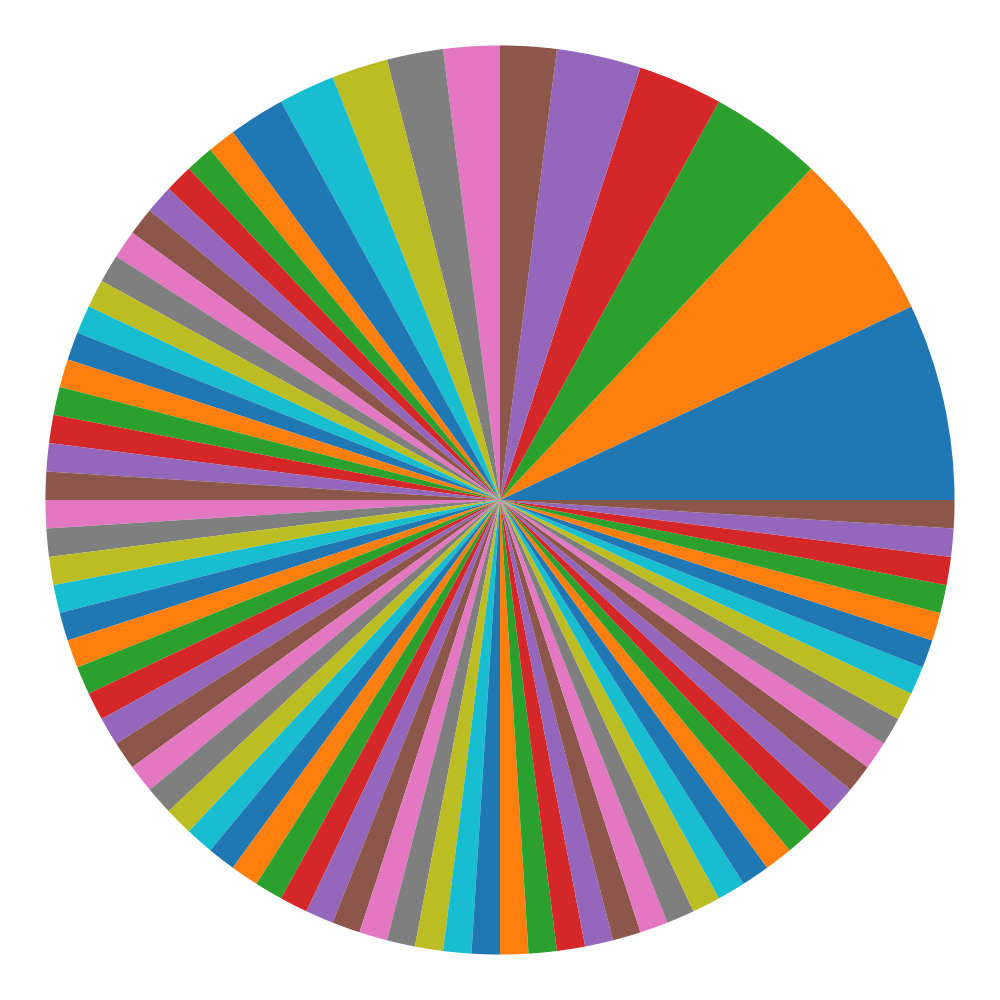
\includegraphics[height=5cm]{graphs/cluster-baseline-8.png}
&
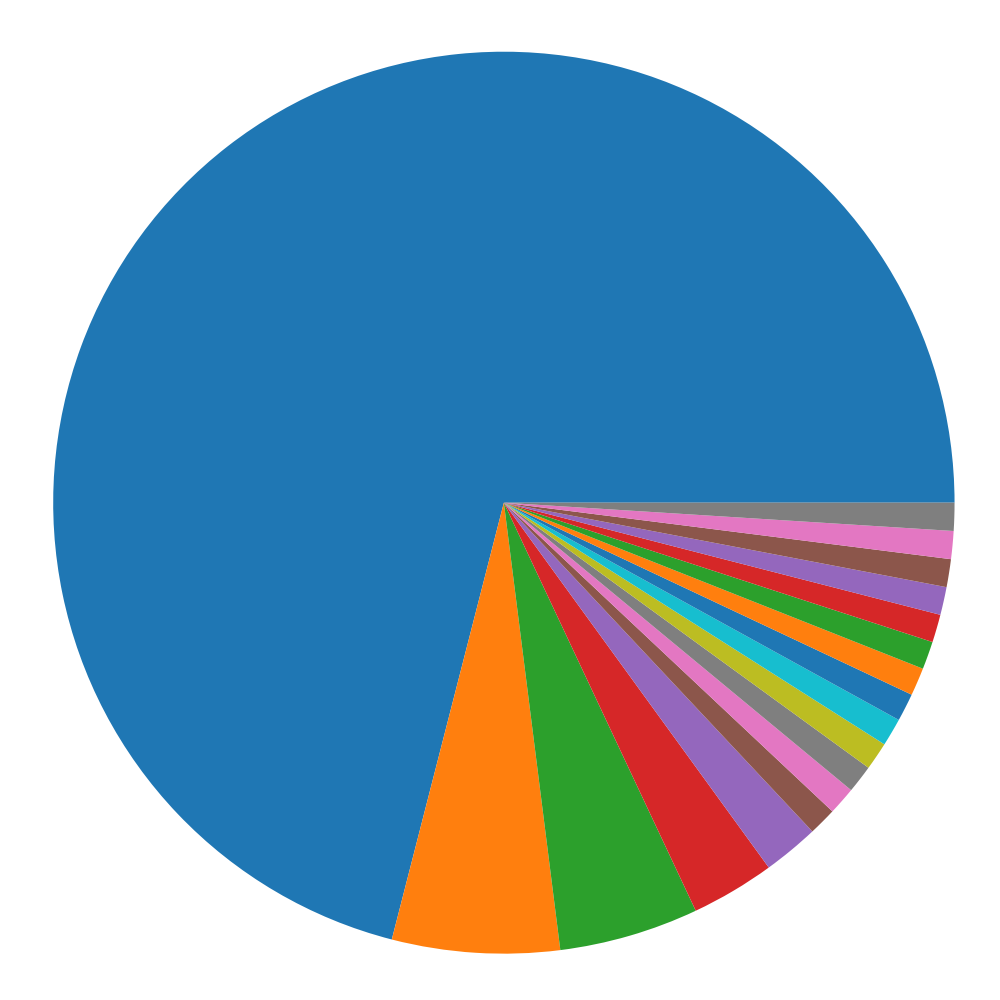
\includegraphics[height=5cm]{graphs/cluster-aggressive-8.png} \\
Before & After
\end{tabular}
\caption{Exercise 8 - Improvement in normalization effectiveness}
\label{fig:improvements-clusters-8}
\end{figure}
